\chapter{Elaborazione sui dati ottenuti}

\begin{figure}
\centering
    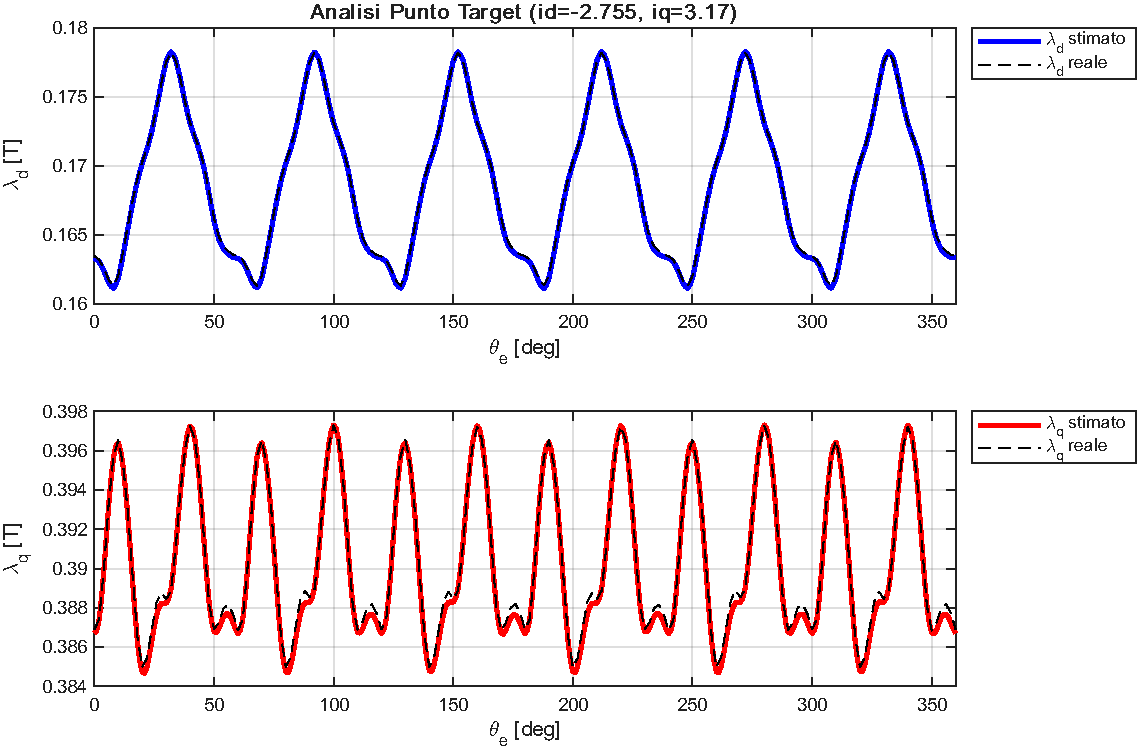
\includegraphics[height=8 cm]{immagini/procedura_misurazione/Confronto_Flussi_PuntoTarget.pdf}
    \caption{Confronto tra il flusso stimato $dq$ e il flusso reale.}
    \label{fig:Flusso_D_vs_Id_ThetaVar_1}
\end{figure}

\section{Analisi dell'errore di stima}
Applicando le formule \ref{eq:flussi_dq2} e \ref{eq:flussi_dq3} è possibile ottenere la stima finale del flusso. Il grafico ottenuto viene riportatoin Figura \ref{fig:Flusso_D_vs_Id_ThetaVar_1}. Come si può notare, nonostante fosse presente un errore nei grafici precedenti  dovuto alla stima della resistenza, questo errore viene in gran parte compensato con la stima finale.\\
Per valutare l'accuratezza della procedura si può stimare l'errore, calcolando la differenza tra $\lambda_d$ reale e stimato (Figura   \ref{fig:Errore_stima_flusso}).
 Per comprendere meglio l'impatto dell'errore sulla stima si può dividere per il valore medio per stimare l'errore percentuale (Figura \ref{fig:Errore_stima_relativo_flusso}).

\begin{figure}
\centering
    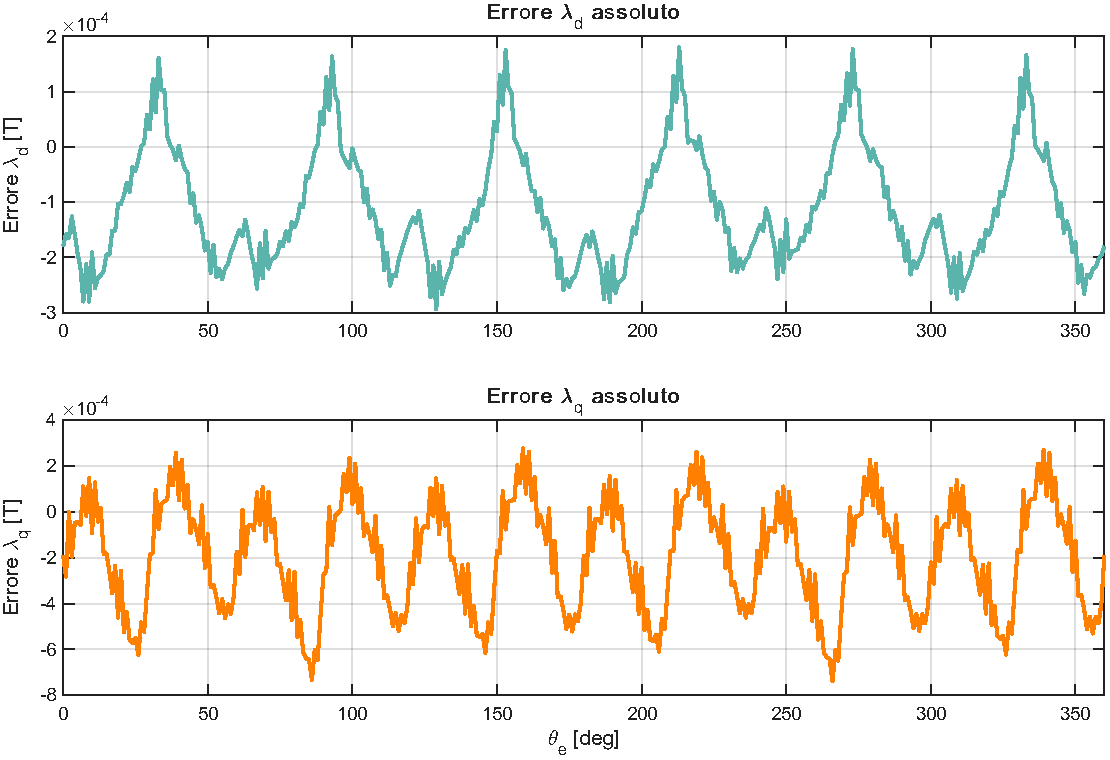
\includegraphics[height=8 cm]{immagini/procedura_misurazione/Errore_stima_flusso.pdf}
    \caption{Differenza tra $\lambda_d$ stimato e reale.}
    \label{fig:Errore_stima_flusso}
\end{figure}


\begin{figure}
\centering
    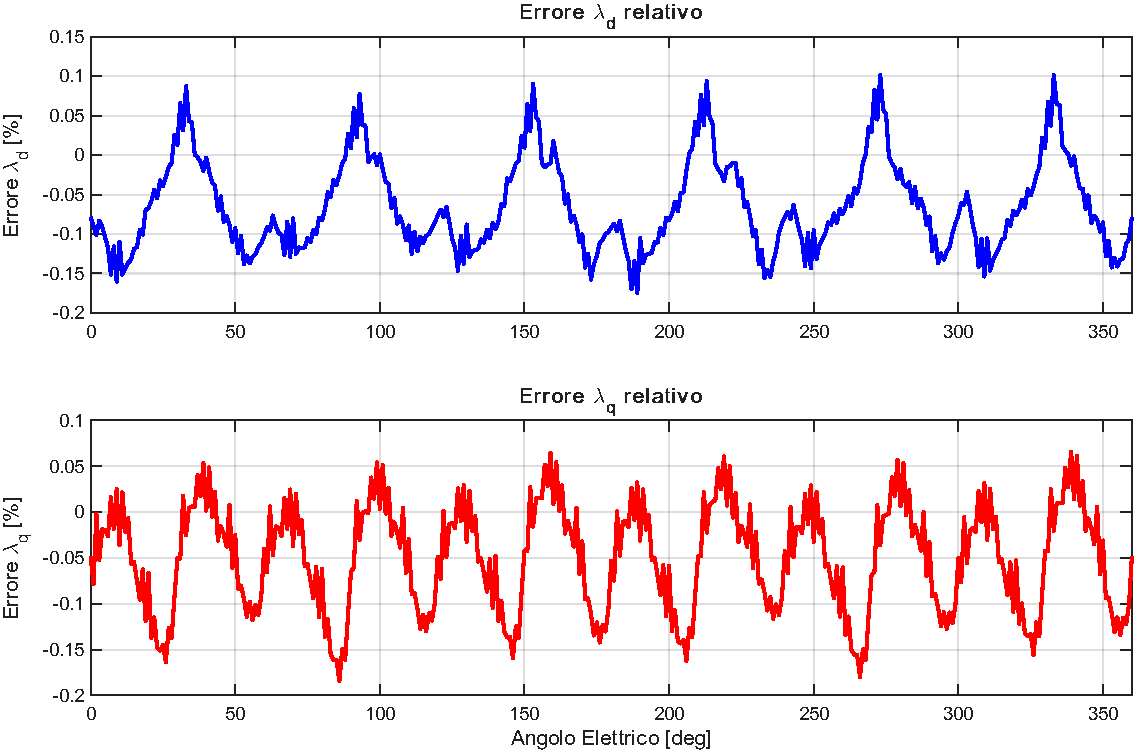
\includegraphics[height=8 cm]{immagini/procedura_misurazione/Errore_stima_relativo_flusso.pdf}
    \caption{Errore percentuale del flusso $\lambda_d$ e $\lambda_q$.}
    \label{fig:Errore_stima_relativo_flusso}
\end{figure}

\section{Introduzione della variazione sulla  resistenza}
Durante la procedura di test, la temperatura del motore aumenta per effetto joule. La variazione della  temperatura comporta una conseguente variazione sulla resistività del rame degli avvolgimenti \cite{Elettrotecnica_1_Principi}.\\ 
La dipendenza della resistività rispetto alla temperatura può essere espressa come segue :
\begin{equation}
    \rho = \rho_0(1+\alpha(T-T_0))
\end{equation}
in cui $T$ è la temperatura effettiva mentre $T_0$ è la temperatura alla quale la resistività è calcolata e $\alpha$ il coefficiente di temperatura caratteristico del materiale.\\
Da tale formula si può ricavare la dipendenza della resistenza dalla temperatura:
\begin{equation}
    R = R_0(1+\alpha(T-T_0))
    \label{eq: res_increase}
\end{equation}
dove $R_0$ è il valore della resistenza alla temperatura $T_0$.\\
Sostituendo i valori standard per il rame e la resistenza statorica del motore sotto test otteniamo:
\begin{equation}
R =  2.726\cdot(1+0.0039\cdot(T-20))  
\end{equation}
Per verificare l'effetto termico, nella simulazione la temperatura cresce linearmente nel tempo. Conseguentemente anche la resistenza aumenta secondo la relazione \ref{eq: res_increase}. \\
Per simulare l'aumento di temperatura del motore dovuta all'effetto joule si è utilizzata una rampa lineare.\\

Si sono provate diverse variazioni di temperatura:
\begin{itemize}
    \item variazione 20°-25°
    \item variazione 20°-30°
\end{itemize}



\begin{figure}
\centering
    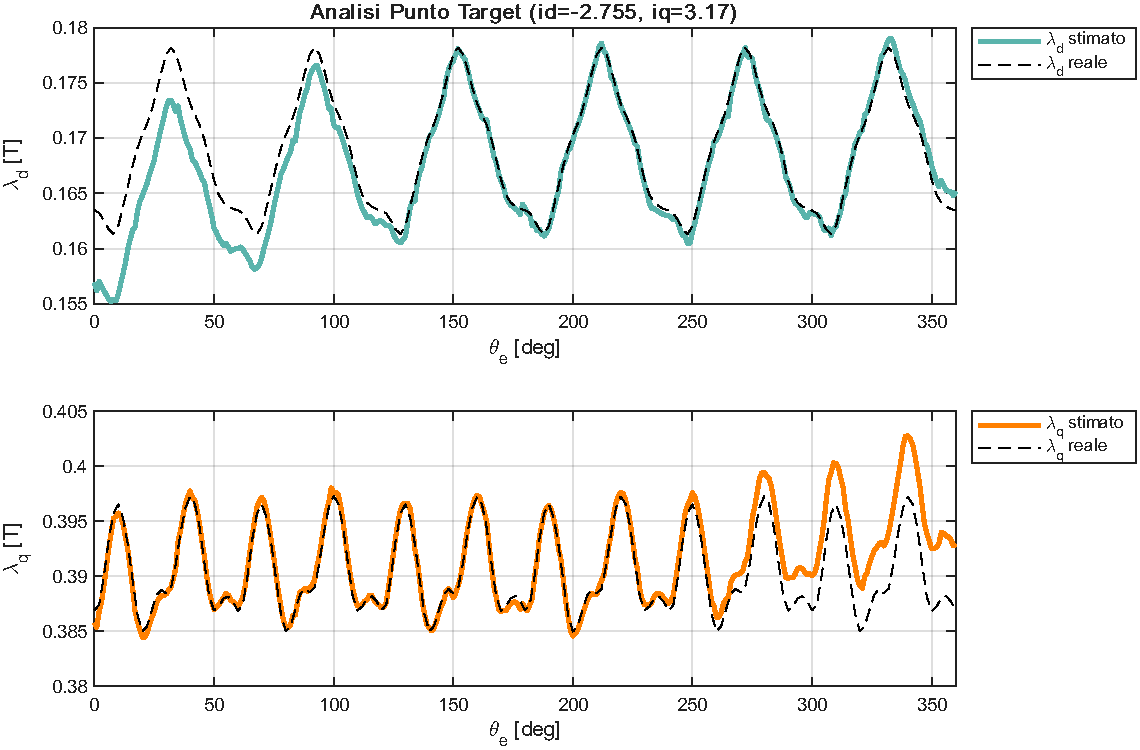
\includegraphics[height=8 cm]{immagini/procedura_misurazione/res_var/Confronto_Flussi_PuntoTarget_res_var.pdf}
    \caption{Stima flusso con resistenza dipendente dalla temperatura.}
    \label{fig:Confronto_Flussi_PuntoTarget_res_var}
\end{figure}

\begin{figure}
\centering
    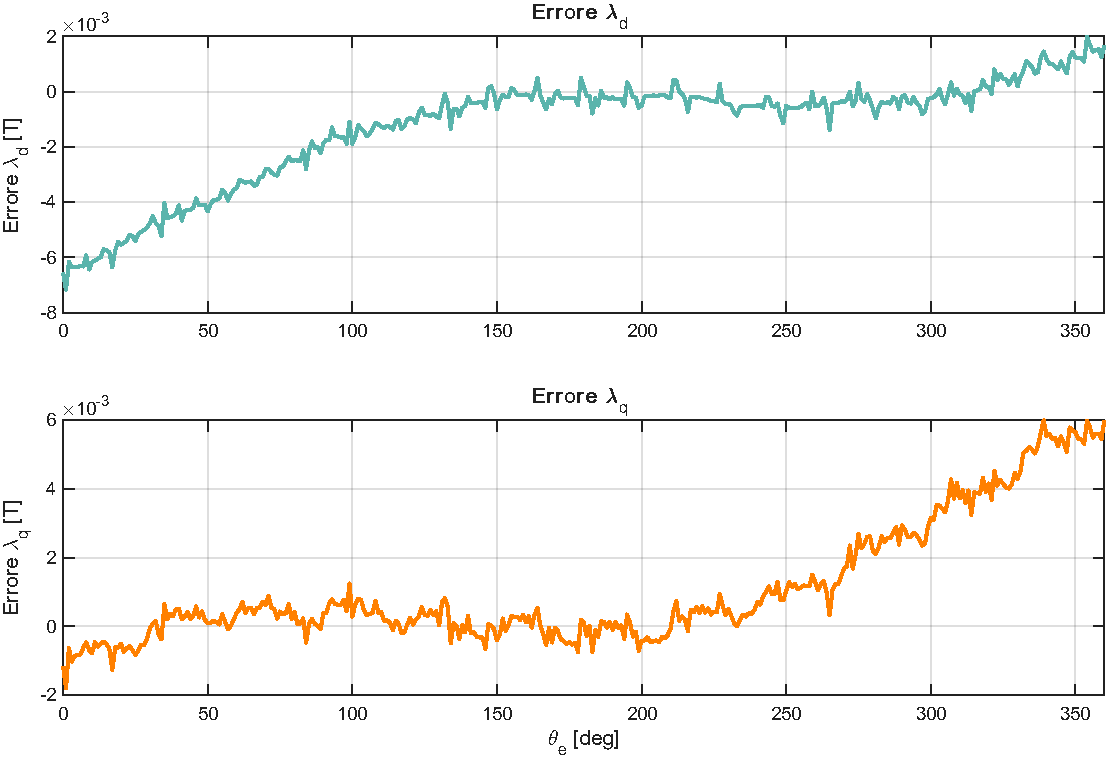
\includegraphics[height=8 cm]{immagini/procedura_misurazione/res_var/Errore_stima_flusso_res_var_500.pdf}
    \caption{Errore di stima del flusso con resistenza variabile.}
    \label{fig:Errore_stima_flusso_res_var_500}
\end{figure}

\subsection{Scelta della posizione iniziale per la raccolta dati}
Inizialmente è stato implementato un algoritmo per la macchina a stati che non prevedeva di iniziare a una specifica posizione angolare.\\
Questo approccio non presenta problemi nel caso in cui il valore della  resistenza statorica rimane costante. Tuttavia, l'introduzione della dipendenza della resistenza dalla temperatura comporta una distorsione molto evidente nella stima del flusso.\\



% ..... COMPLETA

\subsection{Eliminazione dell'errore sul flusso magnetico}
Si osserva come la variazione della resistenza dovuta alla temperatura introduce un errore nella stima (Figura \ref{fig:Confronto_Flussi_PuntoTarget_res_var}).\\
Esaminando l'andamento di questo errore in funzione della posizione si può notare come esso rimane prossimo a zero per la maggior parte dei valori di posizione, ma diverge nel tratto iniziale, nel caso di $\lambda_d$, e finale, nel caso di $\lambda_q$.\\
Per eliminare questo errore di stima i dati della stima di $\lambda_d$ e $\lambda_q$ sono stati post-elaborati utilizzando tre metodi di correzione applicati in successione.
\begin{itemize}
    \item funzione \texttt{polyfit}
    \item fit trigonometrico
    \item correzione degli estremi
\end{itemize}
\subsection{Applicazione della funzione polyfit}
In Figura \ref{fig:Errore_stima_flusso_res_var_500} si può notare come nel primo tratto di $\lambda_d$ e nell'ultimo tratto di $\lambda_q$ sia presente un errore con un andamento circa parabolico.\\ 
Per estrarre questo errore   di stima è stata utilizzata la funzione \texttt{polyfit} di \texttt{MATLAB}. La funzione \texttt{polyfit(x,y,n)} restituisce i coefficienti di un polinomio p(x)  di grado n che costituisce il miglior adattamento per i dati y.\\
Si è scelto 2 come grado del polinomio in quanto l'errore evolve con un andamento circa parabolico.\\
Una volta estratto il polinomio dai dati, viene sottratto per eliminare il trend disatteso.\\
Tuttavia, facendo ciò, viene rimossa anche la componente media. Il valore medio deve così essere nuovamente integrato.\\
Tramite questa procedura di correzione si è ottenuto l'andamento mostrato in Figura \ref{fig:Confronto_Flussi_PuntoTarget_polyfit_500}.



\begin{figure}
\centering
    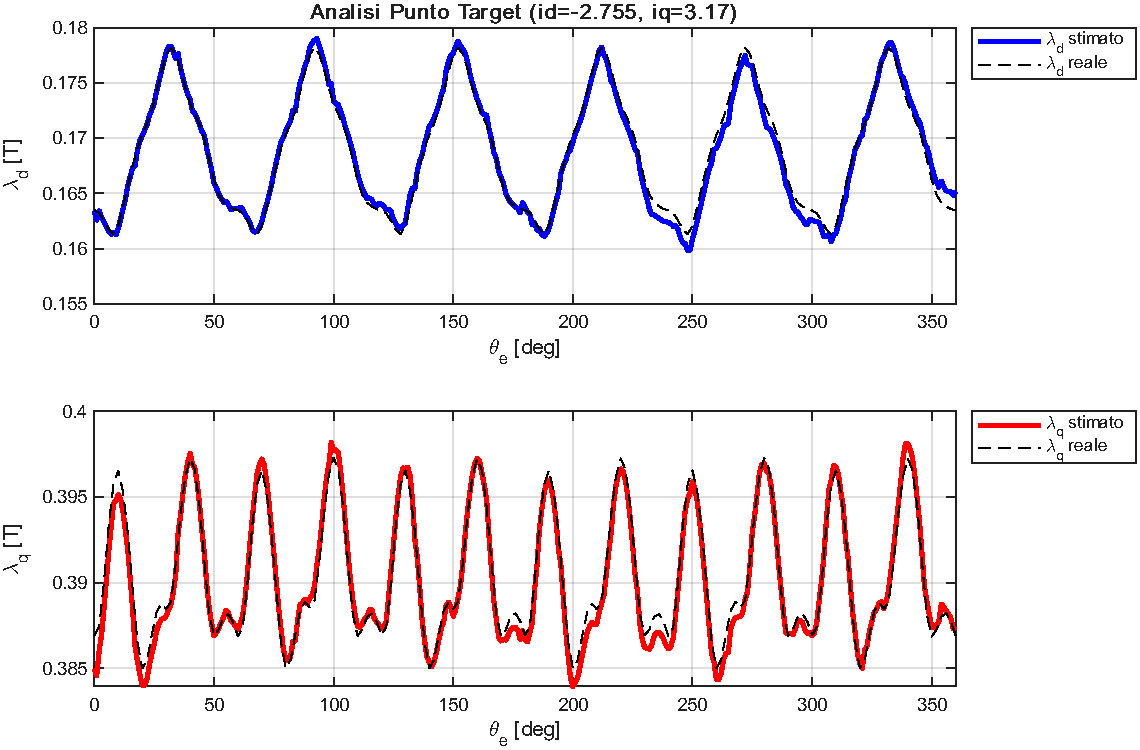
\includegraphics[height=8 cm]{immagini/procedura_misurazione/res_var/Confronto_Flussi_PuntoTarget_polyfit_500.pdf}
    \caption{Confronto dei flussi dopo l'applicazione della funzione \texttt{polyfit}.}
    \label{fig:Confronto_Flussi_PuntoTarget_polyfit_500}
\end{figure}

\begin{figure}
\centering
    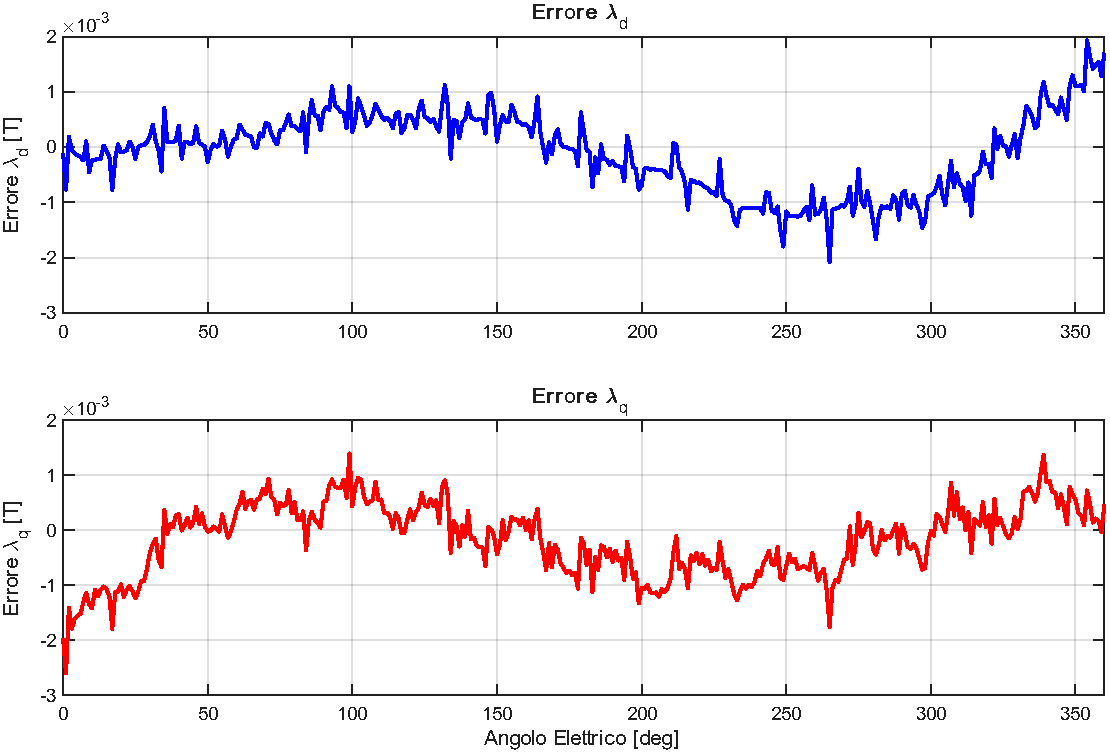
\includegraphics[height=8 cm]{immagini/procedura_misurazione/res_var/Errore_stima_flusso_polyfit_500_.pdf}
    \caption{Errore di stima del flusso dopo l'applicazione della funzione \texttt{polyfit}.}
    \label{fig:Errore_stima_flusso_polyfit_500}
\end{figure}

\subsection{Fit trigonometrico}
Si può notare come sia presente ancora un errore di stima nel tratto finale, sebbene l'estrazione del polinomio abbia migliorato l'accuratezza della stima (Figure \ref{fig:Confronto_Flussi_PuntoTarget_polyfit_500}).  Analizzando la Figura \ref{fig:Errore_stima_flusso_polyfit_500} si osserva come l'errore abbia un andamento simile a quello di una funzione trigonometrica. Tramite un metodo ai minimi quadrati si è quindi estratta la sinusoide che approssima meglio i dati.\\ Come fatto in precedenza si è poi sottratto questa forma d'onda ai dati. \\Il risultato ottenuto è riportato in Figura \ref{fig:Confronto_Flussi_PuntoTarget_armonico_500}.


\begin{figure}
\centering
    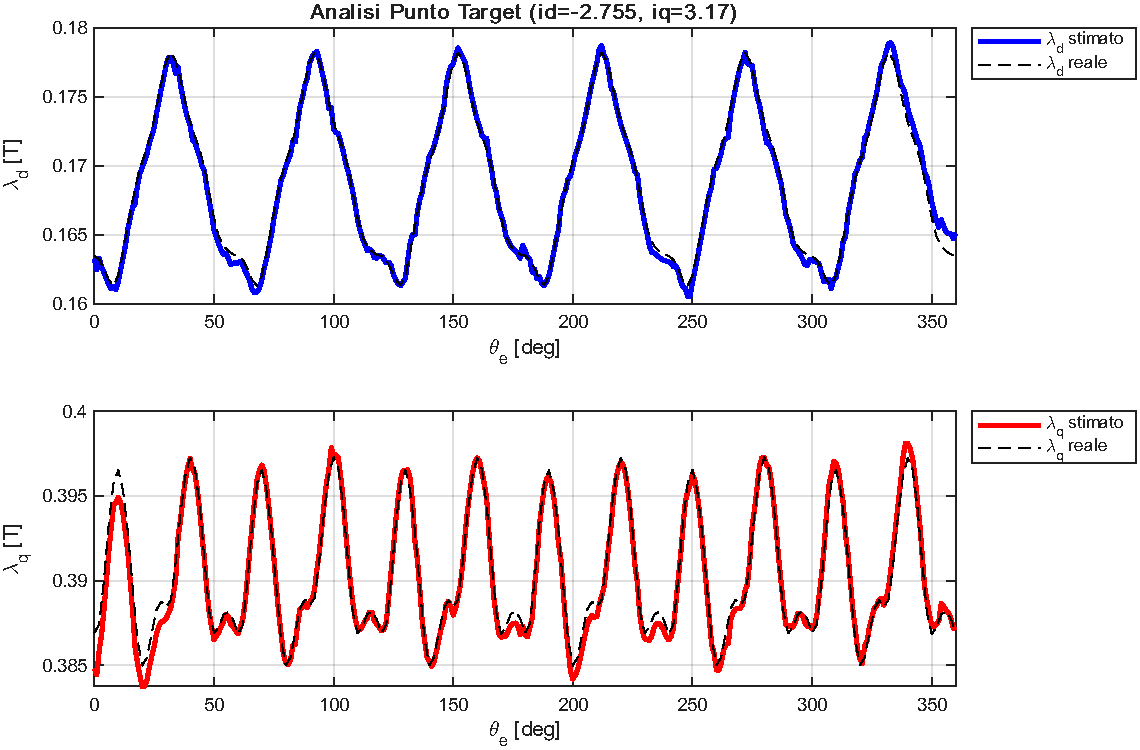
\includegraphics[height=8 cm]{immagini/procedura_misurazione/res_var/Confronto_Flussi_PuntoTarget_armonico_500.pdf}
    \caption{Confronto dei flussi dopo il fitting trigonometrico.}
    \label{fig:Confronto_Flussi_PuntoTarget_armonico_500}
\end{figure}

\subsection{Correzione degli estremi}
Il flusso a 0° deve coincidere necessariamente con il flusso a 360°. Per ovviare a questo problema è stata implementata una correzione usando una curva smooth-step. I risultati sono riportati in Figura \ref{fig:Confronto_Flussi_PuntoTarget_coda_500}.
\begin{figure}
\centering
    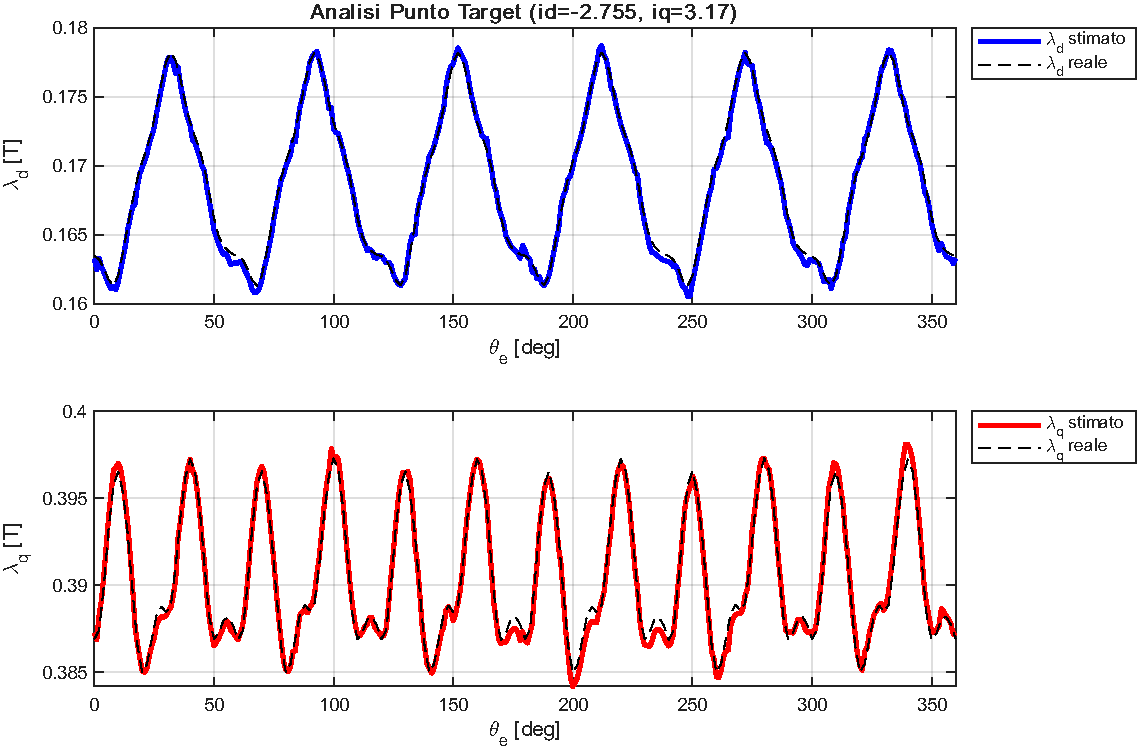
\includegraphics[height=8 cm]{immagini/procedura_misurazione/res_var/Confronto_Flussi_PuntoTarget_coda_500.pdf}
    \caption{Confronto dei flussi dopo la correzione degli estremi.}
    \label{fig:Confronto_Flussi_PuntoTarget_coda_500}
\end{figure}

\subsection{Stima del flusso con range di temperatura 20°-25°}
La stima del flusso nel range 20°-25° risulta accurata. Per validare la procedura, si è stimato il flusso rispetto a 8 punti lungo la curva MTPA.

\begin{table}
    \centering

    \footnotesize

    \bf{Errore di stima su $\lambda_d$}

    \vspace{0.2cm}
    
    \renewcommand{\arraystretch}{1.3}
    \begin{tabular}{
    >{\centering\arraybackslash}m{2.5 cm}
    >{\centering\arraybackslash}m{2.5 cm}
    >{\centering\arraybackslash}m{2.5 cm}
    >{\centering\arraybackslash}m{2.5 cm}
    >{\centering\arraybackslash}m{2.5 cm}
    }
    \arrayrulecolor{black}\toprule
    $\bm{i_d}$ [A]&$\bm{i_q}$ [A]&\textbf{RMSE [T]} &\textbf{Errore medio [\%]} &\textbf{Errore massimo [\%]}\\
    \arrayrulecolor{GRIG}\midrule
        0 & 0
        & $1.42\cdot10^{-4}$
        & 0.06 & 0.13
        \\
    \arrayrulecolor{GRIG}\midrule
        -0.17& 0.57
        & $9.2\cdot10^{-5}$
        & 0.04
        & 0.17
        \\
    \arrayrulecolor{GRIG}\midrule
        
        -0.5& 1.09
        & $1.49\cdot10^{-4}$
        &0.09&0.33
        \\
    \arrayrulecolor{GRIG}\midrule
        
        -0.85& 1.59
        & $2.41\cdot10^{-4}$
        &0.12&0.34
        \\
    \arrayrulecolor{GRIG}\midrule
        
        -1.3& 2.02
        & $2.95\cdot10^{-4}$
        &0.15&0.45
        \\
    \arrayrulecolor{GRIG}\midrule
        
        -1.69& 2.47
        & $3.4\cdot10^{-4}$
        &0.18&0.52
        \\
    \arrayrulecolor{GRIG}\midrule
        
        -2.08& 2.94
        & $3.99\cdot10^{-4}$
        &0.22&0.75
        \\
    \arrayrulecolor{GRIG}\midrule
        
        -2.76& 2.17
        & $3.94\cdot10^{-4}$
        &0.23&0.8
        \\
    \arrayrulecolor{black}\bottomrule
    
    \end{tabular} 
    \caption{Valore dell'errore di stima per punto operativo.}
    \label{tab:Tabella_errore_stima_d}   
\end{table}



\begin{table}
    \centering

    \footnotesize

    \bf{Errore di stima su $\lambda_q$}

    \vspace{0.2cm}
    
    \renewcommand{\arraystretch}{1.3}
    \begin{tabular}{
    >{\centering\arraybackslash}m{2.5 cm}
    >{\centering\arraybackslash}m{2.5 cm}
    >{\centering\arraybackslash}m{2.5 cm}
    >{\centering\arraybackslash}m{2.5 cm}
    >{\centering\arraybackslash}m{2.5 cm}
    }
    \arrayrulecolor{black}\toprule
    $\bm{i_d}$ [A]&$\bm{i_q}$ [A]&\textbf{RMSE [T]} &\textbf{Errore medio [\%]} &\textbf{Errore massimo [\%]}\\
    \arrayrulecolor{GRIG}\midrule
        0 & 0
        & $1.42\cdot10^{-4}$
        & 0.06 & 0.13
        \\
    \arrayrulecolor{GRIG}\midrule
        -0.17& 0.57
        & $9.2\cdot10^{-5}$
        & 0.04
        & 0.17
        \\
    \arrayrulecolor{GRIG}\midrule
        
        -0.5& 1.09
        & $1.49\cdot10^{-4}$
        &0.09&0.33
        \\
    \arrayrulecolor{GRIG}\midrule
        
        -0.85& 1.59
        & $2.41\cdot10^{-4}$
        &0.12&0.34
        \\
    \arrayrulecolor{GRIG}\midrule
        
        -1.3& 2.02
        & $2.95\cdot10^{-4}$
        &0.15&0.45
        \\
    \arrayrulecolor{GRIG}\midrule
        
        -1.69& 2.47
        & $3.4\cdot10^{-4}$
        &0.18&0.52
        \\
    \arrayrulecolor{GRIG}\midrule
        
        -2.08& 2.94
        & $3.99\cdot10^{-4}$
        &0.22&0.75
        \\
    \arrayrulecolor{GRIG}\midrule
        
        -2.76& 2.17
        & $3.94\cdot10^{-4}$
        &0.23&0.8
        \\
    \arrayrulecolor{black}\bottomrule
    
    \end{tabular} 
    \caption{Valore dell'errore di stima per punto operativo.}
    \label{tab:Tabella_errore_stima_q}   
\end{table}





\section{Implementazione dell'algoritmo di stima multiplo}
infine risulta necessario iterare la procedura di stima per ogni coppia di correnti della griglia.\\
I risultati finali vengono salvati all'interno di una mappa.

\begin{comment}
Si è verificato quindi la stima del flusso introducendo questo fenomeno ( Figura \ref{fig:Confronto_Flussi_PuntoTarget_Res}).

\begin{figure}[H]
\centering
    
\includegraphics[height=8 cm]{immagini/flusso_concatenato/Confronto_Flussi_PuntoTarget_Res.pdf}
    \caption{Confronto tra il flusso stimato $dq$ e il flusso reale con variazione resistiva.}
    \label{fig:Confronto_Flussi_PuntoTarget_Res}
\end{figure}

\end{comment}
\begin{comment}
\section{Creazione modello utilizzando le induttanze differenziali}
Si può implementare il modello fisico del motore utilizzando le induttanze differenziali.\\
Dalle equazioni elettriche del motore si ottiene che:

\begin{equation}
\begin{dcases}
    \frac{d\lambda_d}{dt} =u_d- Ri_d+\omega_{me}\lambda_q\\
    \frac{d\lambda_q}{dt} =u_q -Ri_q-\omega_{me}\lambda_d
\end{dcases}
\label{eq:equazioni_elettriche}
\end{equation}

Sostituendo l'espressione delle derivate del flusso ottenute precedentemente (\ref{eq:induttanze_diff_elet}) nelle equazioni \ref{eq:equazioni_elettriche}, si ottiene che:

\begin{equation}
\begin{dcases}
    \frac{di_d}{dt} =\frac{1}{l_d}[ u_d- Ri_d+\omega_{me}\lambda_q-l_{dq}\frac{di_q}{dt}-l_{d\theta}\omega_m]\\
    \frac{di_q}{dt} =\frac{1}{l_q}[ u_q- Ri_q-\omega_{me}\lambda_q-l_{qd}\frac{di_q}{dt}-l_{q\theta}\omega_m]
\end{dcases}
\label{eq:equazioni_elettriche2}
\end{equation}

Le induttanze differenziali possono essere calcolate applicando la funzione "gradient" di MATLAB.\\
Tuttavia, si è notato come questo approccio porti a un maggiore disturbo sulle correnti  $i_d$ e $i_q$.
Ciò si traduce in un errore di stima con la procedura di stima illustrata nel Paragrafo \ref{sec:stima_flusso}.
\end{comment}
